\chapter{Practical Applications of Refactoring Detection}
\label{ChPracticalApplications}

Throughout this thesis we discussed tools to mine refactorings from version histories and empirical studies that benefit from such techniques. In this chapter, we discuss three practical applications of such tools.
We do not intend to thoroughly discuss all possible applications, but rather to exemplify that some relevant problems faced by development teams can be tackled with the help of such tools.
Particularly, RefDiff's multi-language design is an important advantage for the practical applications described in this chapter, as software projects are developed using different programming languages.


\section{Refactoring-aware Diff}
\label{SecRefactoringDiff}


One of the challenges developers face when refactoring, as reported in an in-depth study by \cite{kim-tse-2014}, is the difficulty of reviewing code after refactoring.
This is illustrated by the following comment from one of the developers interviewed by Kim~et~al.:\margin

\noindent{\em \quotes{It (refactoring) typically increases the number of lines/files involved in a check-in. That burdens code reviewers and
increases the odds that your change will collide with someone
else's change.}}\margin

In fact, version control systems are usually sensitive to rename and move refactoring,
which makes it hard for developers to understand code changes, specially when refactorings are applied interleaved with other modifications in the system.


%intellij-community ce5f9ff
\begin{figure}[htpb]
\centering
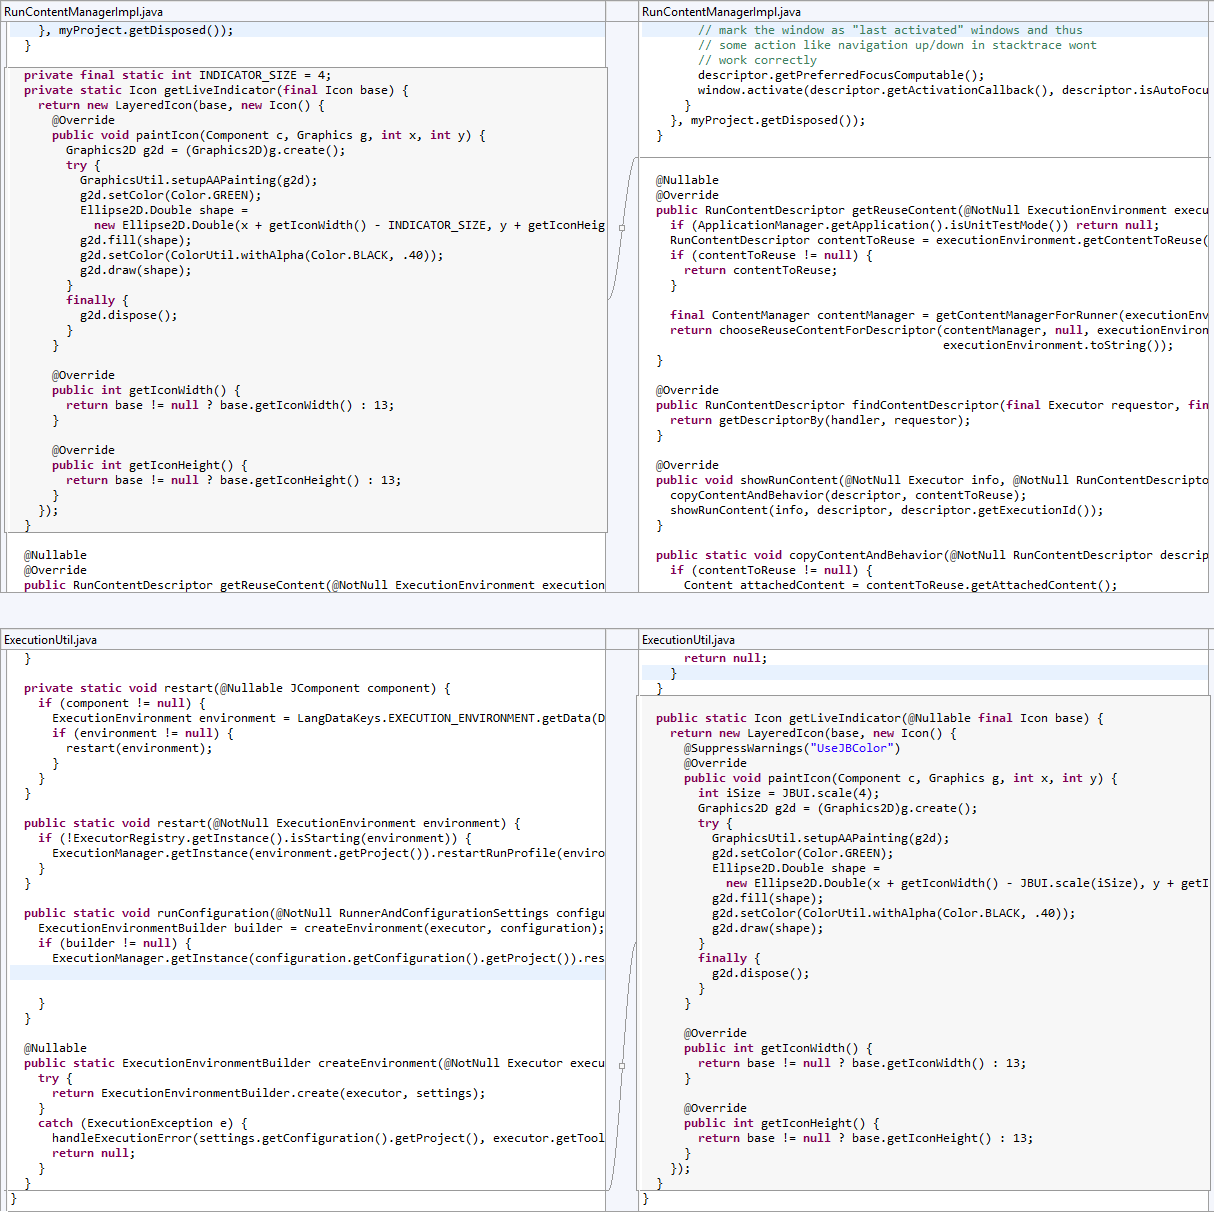
\includegraphics[width=\linewidth]{img/c1.png}
\caption{Typical diff visualization of a code change containing a moved method}
\label{FigRwDiff1}
\end{figure}

As a concrete example, consider the code changes presented in Figure~\ref{FigRwDiff1}, which are taken from the \url{intellij-community} repository. In this figure, we present the code diff between two changed files. In the first one, \texttt{RunContentManagerImpl.java}, a large code block was removed, whilst in the second file (\texttt{ExecutionUtil.java}) a large code block was added. With a thoroughly analysis, we can note that the code removed from \texttt{RunContentManagerImpl.java} was actually moved to \texttt{ExecutionUtil.java}, i.e., the method \texttt{getLiveIndicator} was moved.
However, this is not immediately obvious to a developer reviewing these changes, specially considering that there might be many other changed files in the commit. Moreover, although one can identify with some effort that the method \texttt{getLiveIndicator} has been moved, it will be much more difficult to identify small changes made to its body in this visualization.

\begin{figure}[bp]
\centering
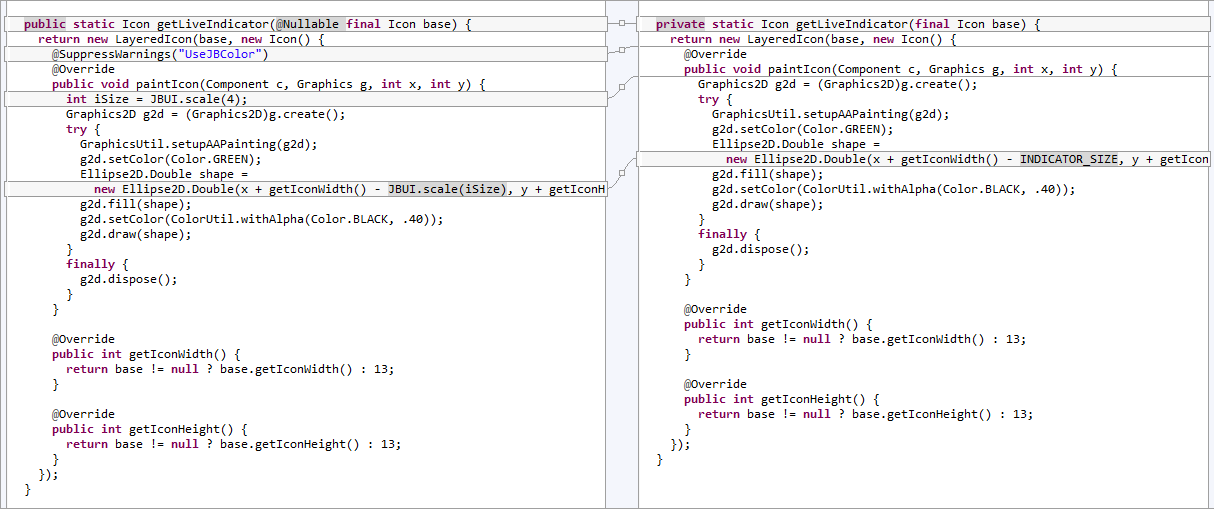
\includegraphics[width=\linewidth]{img/c2.png}
\caption{Diff visualization focused on the moved method}
\label{FigRwDiff2}
\end{figure}

In contrast, consider the diff visualization presented in Figure~\ref{FigRwDiff2}. In this case, the diff is focused in the method that was moved, \texttt{getLiveIndicator}, before and after the change. We can clearly see that some changes have been made to the body of \texttt{getLiveIndicator}. Specifically, the annotations \texttt{@Nullable} and \texttt{@SuppressWarnings} were introduced, a new local variable \texttt{iSize} was declared, and the expression passed as the first argument to the \texttt{Ellipse2D.Double} constructor was changed.
All these changes are very hard to note in a traditional diff visualization, such as the one from Figure~\ref{FigRwDiff1}, but are easily discernible when we present the moved method compared with its counterpart.
Other refactoring types might benefit from such idea as well.
As a second example, it would also be convenient to highlight the differences between an extracted method and its originating code. This way, it would become easier to identify new statements added.
A similar reasoning can be applied to Move Class, Inline Method, and other refactoring types.



Thus, we can improve diff visualization using the information about the refactorings detected in commits, using a tool such as RefDiff.
We expect that such refactoring-aware diff visualization solution would improve developers' ability to discern and understand code changes in the presence of refactorings, enabling them to concentrate on behavioral changes rather than on code modifications resulting from refactorings.


\section{Tracking changes of a code element}
\label{SecAppTrackChanges}

Although refactoring is very important to maintain a software system, it can make it harder to track code changes in the history, specially at the method/function level.
% https://github.com/facebook/react/commit/63aa7259b9f48886af545afcc06c29acf225b05f
For example, consider the \texttt{getReactRootElementInContainer} function from React project, depicted in Figure~\ref{FigGitBlameReact}.
\begin{figure}[b]
\centering
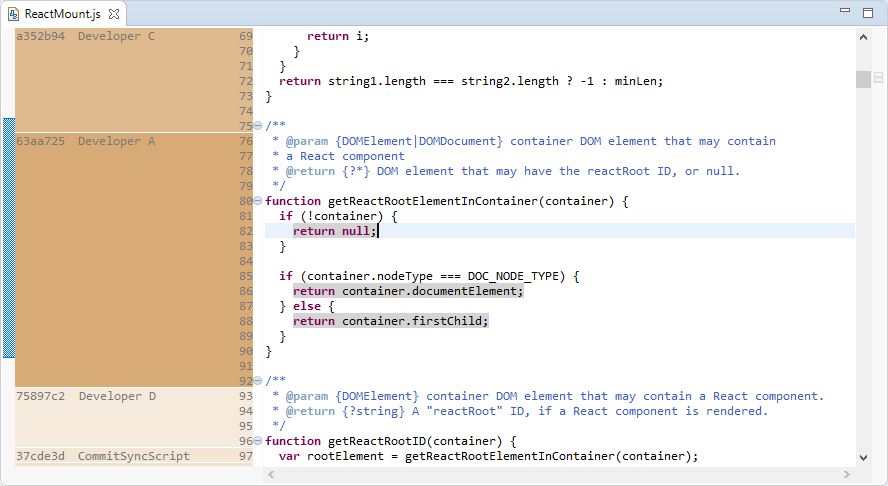
\includegraphics[width=\linewidth]{img/git-blame-react.png}
\caption{\textit{git-blame} visualization of the \texttt{ReactMount.js} file from React project, showing that function \texttt{getReactRootElementInContainer} was last modified by Developer~A}
\label{FigGitBlameReact}
\end{figure}
Suppose one is investigating the history of that function to find out who introduced the conditional statement in lines 85--89. Developers typically use the \textit{git-blame} tool for such tasks, as it shows what revision and author last modified each line of code of a file. However, although the \textit{git-blame} output shows that Developer~A was the last developer who modified the lines of code within \texttt{getReactRootElementInContainer}, this information may mislead one to think that he is the author of the function.
In fact, a deeper analysis of the history reveals that Developer~A actually moved the function from file \texttt{getReactRootElementInContainer.js} to \texttt{ReactMount.js}.
Thus, to find the actual author of those lines of code, one should inspect the history of changes of the original file of the function. Figure~\ref{FigGitBlameReactActualAuthor} shows that the conditional in lines 85--89 was actually introduced by Developer~B.


\begin{figure}[htbp]
\centering
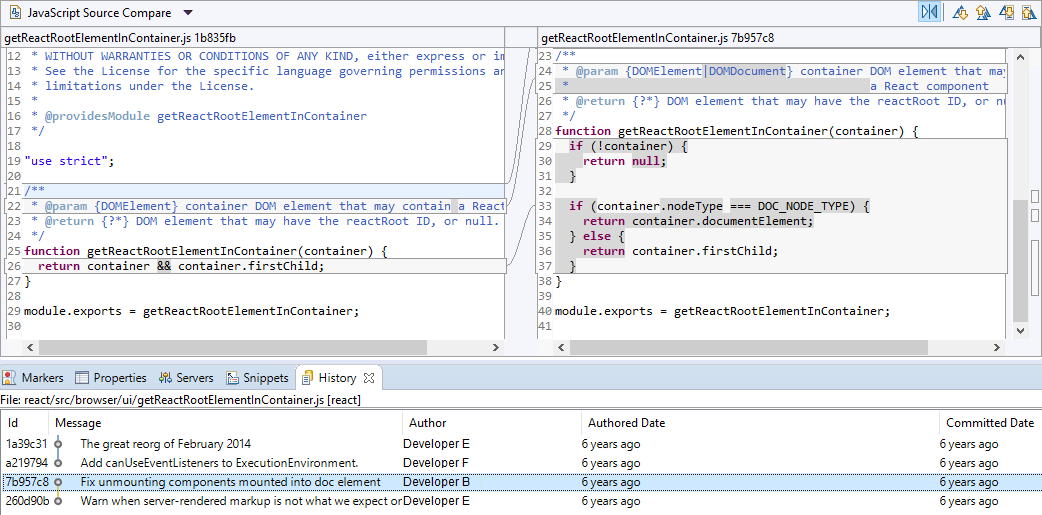
\includegraphics[width=\linewidth]{img/git-blame-react-actual-author.png}
\caption{Diff visualization of the commit in witch the conditional inside function \texttt{getReactRootElementInContainer} was introduced, showing that the actual author is Developer~B}
\label{FigGitBlameReactActualAuthor}
\end{figure}

In summary, in the example above, the \textit{Move Function} refactoring split the history of \texttt{getReactRootElementInContainer}, making it harder to trace back the author of each line of code.
The frequency in which such situations occur makes this problem even more important. \cite{icse2018} studied the extent in which MSR approaches that relies on tracking
the changes along all versions of each individual methods (or classes) are affected by refactorings, i.e., a method rename or move can be misinterpreted as the disappearance of a method and the appearance of a brand new one.
The authors found that between 10\% and 21\% of method-level changes and 2\% and 15\% of class-level changes may introduce a discontinuity in their histories.
Moreover, 25\% of the code elements have at least one discontinuity in their histories.

For these reasons, this problem is a potential application of refactoring detection techniques. If we know the refactorings applied in the system, we can keep track of all moves/renames applied to each code element and reconstruct its full history.
Moreover, this would enable us to provide an improved \textit{git-blame} that shows the last modification of each line of code but is not susceptible to code movement.



\section{Resolving merge conflicts}
\label{SecAppMerge}

Another challenge developers face when refactoring, also reported by \cite{kim-tse-2014}, is the difficulty of merging code.
In software projects, usually several developers work in parallel fixing bugs and adding features to the system.
Thus, the different changes introduced by each developer should be integrated together in the same code base, in a process called as merging code.
In many cases, merging can be done automatically by version control systems, which provide algorithms for such task.
However, when different changes are made to the same lines of code, these algorithms report a conflict, and merge must be done manually.
High-level refactoring operations amplify the odds that merge conflict occurs, because they usually involve movement of large chunks of code.
In fact, a recent study on the relationship between refactoring and merge conflicts shows that refactoring operations are involved in at least 22\% of merge conflicts~\citep{mahmoudi2019refactorings}.

\begin{figure}[htbp]
\centering
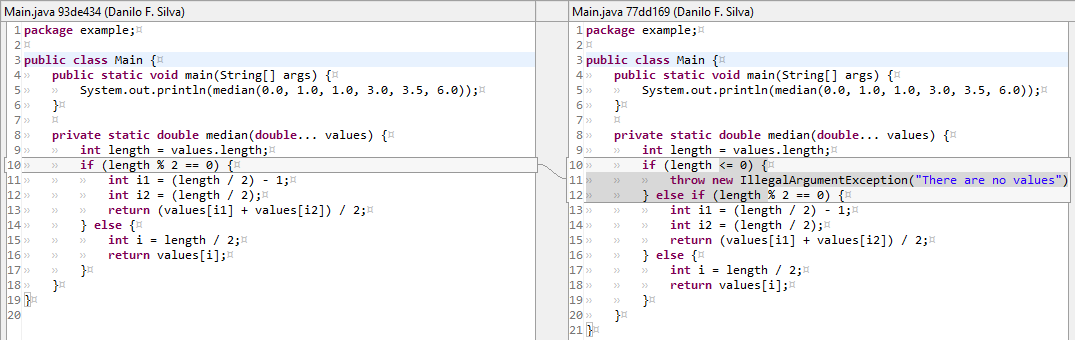
\includegraphics[width=\linewidth]{img/merge-ex-diff1.png}
\caption{Hypotetical change made by first developer: Test if \texttt{length} is zero}
\label{FigMergeExDiff1}
\end{figure}

\begin{figure}[htbp]
\centering
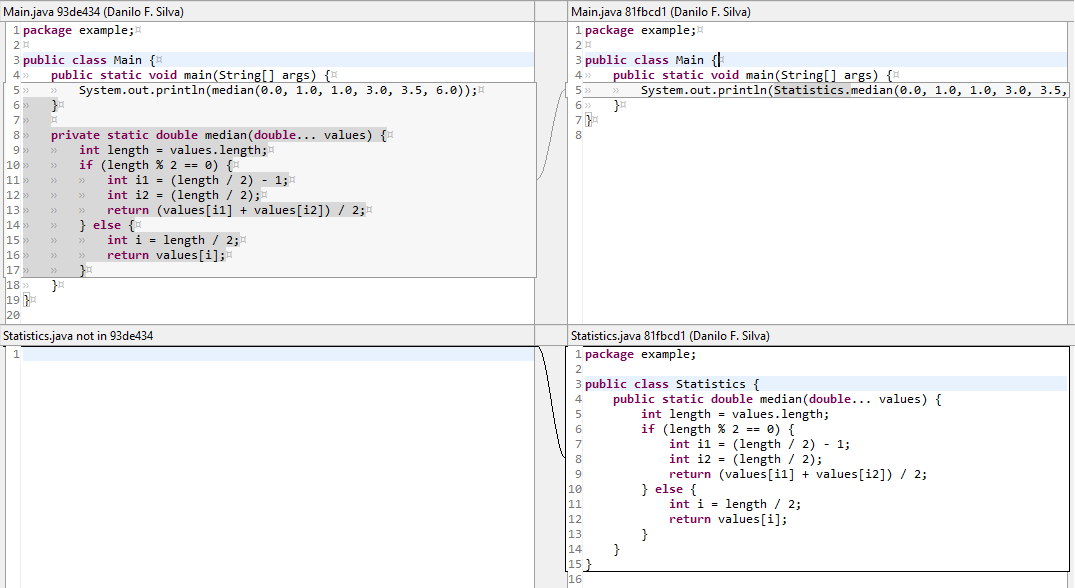
\includegraphics[width=\linewidth]{img/merge-ex-diff2.png}
\caption{Hypotetical change made by second developer: Move method \texttt{median} from class \texttt{Main} to class \texttt{Statistics}}
\label{FigMergeExDiff2}
\end{figure}

\begin{figure}[htbp]
\centering
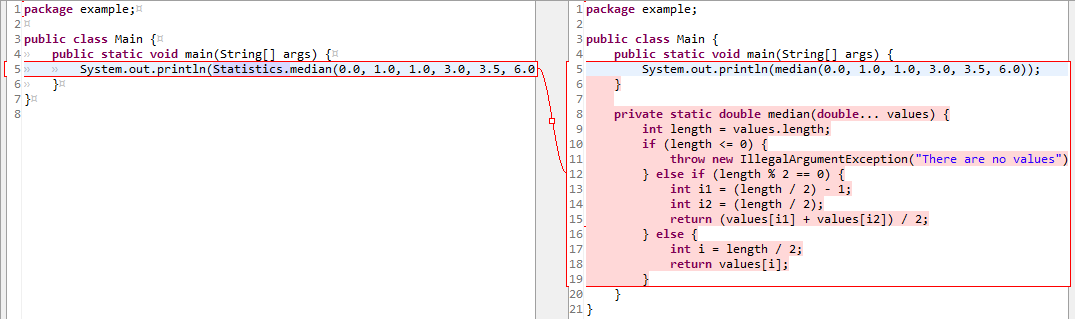
\includegraphics[width=\linewidth]{img/merge-ex-conflict.png}
\caption{When we merge the changes from figures \ref{FigMergeExDiff1} and \ref{FigMergeExDiff2} we get a conflict}
\label{FigMergeExConflict}
\end{figure}

We can illustrate such issues with the following scenario. Consider the example code diff in Figure~\ref{FigMergeExDiff1}, in which a first developer modified method \texttt{median} from class \texttt{Main}, adding a clause that throws an exception when \texttt{length} is zero. Now, suppose that a second developer, working in parallel, decides to move method \texttt{median} from class \texttt{Main} to a new class \texttt{Statistics}, such as depicted in Figure~\ref{FigMergeExDiff2}.
Note that the first developer modified line 10 from file \texttt{Main.java}, while the second developer modified/deleted lines 5--17 from the same file.
Thus, when we merge both changes, we will get a conflict, as depicted in Figure~\ref{FigMergeExConflict}.
In this case, to resolve the merge conflict, one must apply the same logic introduced by the first developer to the \texttt{median} method that is now in class \texttt{Statistics}, and accept the left side of the code from Figure~\ref{FigMergeExConflict} in \texttt{Main.java}.
Note that, even in that small hypothetical example, resolving merge conflicts is tricky and error-prone.
Thus, large-scale refactorings have the potential to make merging changes extremely complicated.

However, we can improve merging algorithms if we know the refactorings applied to the code.
For example, \cite{dig2008effective} proposed a refactoring-aware version control system that is able to resolve merge conflicts caused by refactorings using the following strategy: it identifies the refactorings applied between revisions, undo the refactorings, apply regular textual merge algorithms, and finally apply the refactorings again.
As another example, \cite{cavalcanti2017evaluating} propose an improvement in semistructured merge algorithms that relies on the Levenshtein distance to find renamed code elements. This way, it avoids reporting merge conflicts when a developer renames a method whose body is changed by other developer in parallel.
\cite{shen2019intellimerge} also propose a refactoring-aware merging technique based on a semistructured representation of the source code.
Their tool, called IntelliMerge, first transforms the source code of each revision involved in the merge process into Program Element Graphs (PEGs).
Then, nodes from these graphs are matched with their base version, i.e., in this step refactorings such as \emph{Move} and \emph{Rename} are found.
Finally, textual merge is applied individually for each node, considering the matchings found in the previous step.
The aforementioned tools depend on finding refactorings applied between revision. Thus, they are another direct application of refactoring detection approaches such as RefDiff.


